\documentclass[../00_Main.tex]{subfiles}
\begin{document}

\subsection{Conceptual Design}
The proposed solution is a hybrid electro-acoustic emulation system. It integrates a digital signal processing platform with a physical analog transduction architecture to simulate electrophysiological activity in a phantom head mimicking EEG signals.

\subsubsection{Software and Hardware Subsystems}
The system is conceptualized as two distinct but synchronized subsystems:

\begin{enumerate}
    \item \textbf{The Digital Control Unit (Software):} A desktop application responsible for the deterministic synthesis of waveforms and real-time visualization of acquired data for contrast. This subsystem acts as the signal generator controller, utilizing the host computer's audio sound card as a high-fidelity DAC source to output precise voltage fluctuations at set frequencies. The software has also included functionality to parse and playback clinical EEG data from EDF files, allowing for realistic simulation scenarios.
    
    \item \textbf{The Analog Transduction Unit (Hardware):} A physical interface designed to convert the line-level audio output from the PC into microvolt-scale ($\mu V$) potentials compatible with medical acquisition equipment. The audio output from the PC sound card is first splitted into two mono channels (left and right), each routed to an independent signal amplifier circuit containing a non-inverting opamp and potentiometer to control the gain of the signal. The resulting signals are then injected into the phantom head model, composed of a conductive volume filled with gelatine where the audio jacks are placed as dipoles. Electrodes positioned on the surface of the phantom head capture the resulting potential differences, which can then be acquired by an EEG acquisition system and fed back into the software for analysis.
\end{enumerate}

\subsubsection{High-Level Block Diagram}
Figure~\ref{fig:block_diagram} illustrates the high-level architecture of the proposed solution, highlighting the interaction between the software and hardware components.

\begin{figure}[h]
    \centering
    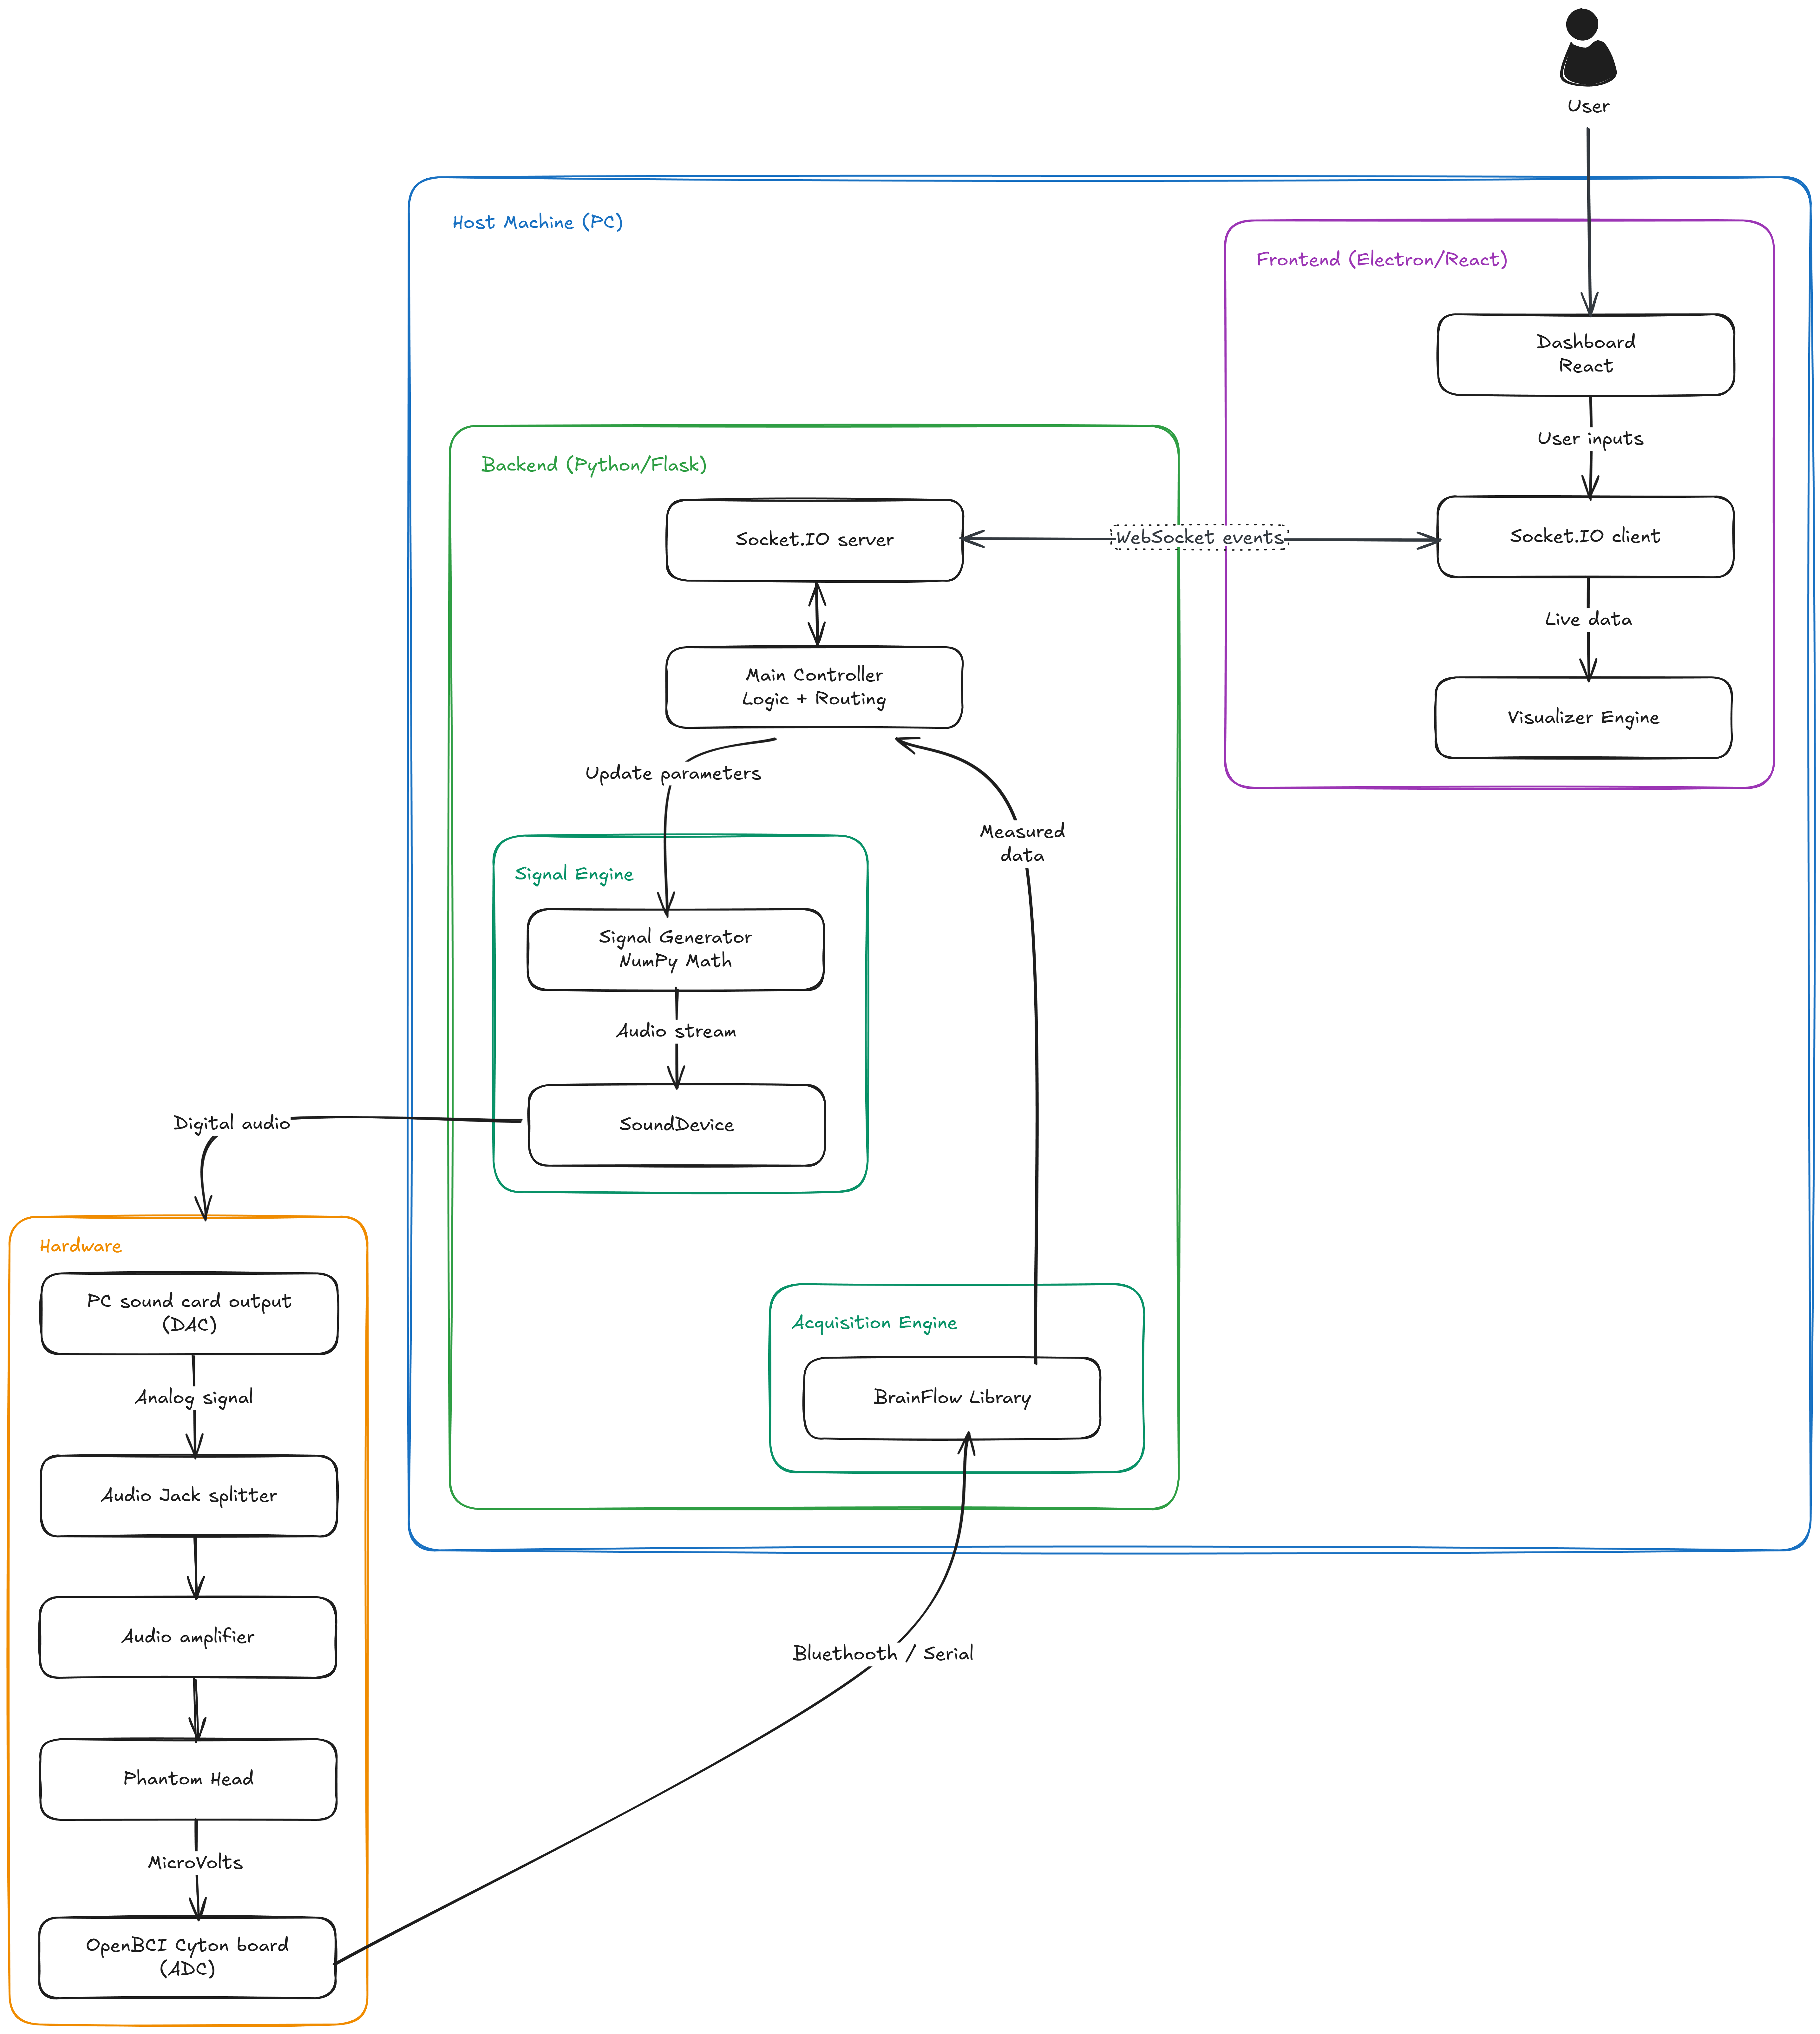
\includegraphics[width=\textwidth]{../../02_Images/high_level_block_diagram.png}
    \caption[High-level block diagram of the solution]{High-level block diagram of the proposed EEG signal emulation system, showing the flow from user configuration to signal acquisition.}
    \label{fig:block_diagram}
\end{figure}

\subsubsection{System Data Flow}
\begin{enumerate}
    \item \textbf{User Configuration:} The user defines the desired EEG parameters via the dashboard interface.
    \item \textbf{Digital Synthesis:} The Python backend generates a discrete-time signal array.
    \item \textbf{D/A Conversion:} The PC's audio DAC reconstructs the continuous analog signal.
    \item \textbf{Channel Splitting:} Each audio output is splitted into two mono signals, obtaining the channels left and right.
    \item \textbf{Signal Conditioning:} Each channel is processed with a non-inverting opamp and potentiometer for amplification.
    \item \textbf{Dipole Construction:} The channels are routed to the phantom head model as dipoles using audio jack terminals.
    \item \textbf{Volume Conduction:} The signal is injected into the phantom head, establishing an electric field distribution.
    \item \textbf{Acquisition:} The EEG electrodes detect the potential difference on the phantom's surface, closing the loop.
\end{enumerate}


\subsection{System Architecture}

\subsubsection{Software Architecture Pattern}

The software platform implements a local client-server architecture encapsulated within a desktop runtime environment. Unlike traditional monolithic desktop applications (compiled in C++ or C\#) or purely cloud-based web applications, this solution adopts a hybrid approach known as a decoupled monolith.

Using this architecture, the presentation layer (frontend) and the logic layer (backend) execute as independent processes on the host machine, communicating via a local network loopback interface. This design leverages the visualization capabilities of modern web technologies while retaining the raw computational power and hardware access of a native Python environment.

The designed architecture is composed of three primary layers:

\begin{enumerate}
    \item \textbf{The Client Container (Electron):} The application is wrapped in Electron, a framework that embeds a Chromium browser instance and a Node.js runtime. Electron serves two critical functions:
    \begin{itemize}
        \item \textbf{Process Orchestration:} Upon execution, the Electron main process spawns the Python backend as a child subprocess, ensuring that the server starts and terminates in sync with the application window.
        \item \textbf{Native Integration:} It provides the application with native OS capabilities (file system access for exporting EDFs, window management, etc.) that are restricted in standard web browsers.
    \end{itemize}

    \item \textbf{The Application Server (Python Flask):} The core logic resides in a distinct Python process managed by the Flask micro-framework. Its responsibilities include:
    \begin{itemize}
        \item \textbf{Mathematical Synthesis:} executing the signal generation algorithms via \texttt{NumPy}.
        \item \textbf{Hardware Abstraction:} managing the audio stream (via \texttt{sounddevice}) and the OpenBCI connection (via \texttt{BrainFlow}).
        \item \textbf{EDF Management:} parsing and exporting clinical data using \texttt{pyedflib}.
    \end{itemize}

    \item \textbf{The Communication Bridge (Socket.IO):} To satisfy the non-functional requirement of low latency (NFR-01), the system bypasses standard HTTP REST protocols. Instead, it utilizes Socket.IO to establish a persistent, bidirectional WebSocket connection between the React frontend and the Flask backend. This event-driven protocol allows the server to push high-frequency signal data (60 packets/second) to the visualizer without the overhead of HTTP headers or polling.
\end{enumerate}

This architecture ensures Separation of Concerns (SOC): the frontend remains responsive even if the backend performs intensive signal processing, as the user interface and the audio engine run on separate threads and memory spaces.


\subsubsection{Technology Stack}
\begin{itemize}
    \item \textbf{Frontend:} React, TypeScript, Vite.
    \item \textbf{Backend:} Python, Flask, Socket.IO, NumPy, Brainflow.
    \item \textbf{Communication:} WebSocket (Socket.IO) event-driven protocol.
\end{itemize}
\subsection{Software Platform}

\subsubsection{Signal Generation Engine}
\subsubsection{User Interface Design}
\subsection{Hardware Architecture}

\subsubsection{Phantom Head Building Specifications}
Detailed methodology for constructing the full phantom head:
\begin{itemize}
    \item Gelatine formulation.
    \item Assembly of the phantom head model.
    \item 10{-}20 System electrode placement strategy.
\end{itemize}

\biblio~% Needed for referencing to working when compiling individual subfiles - Do not remove
\end{document}